\documentclass[11pt]{article}
\usepackage[margin=1in]{geometry}
\usepackage{graphicx,booktabs,float}
\PassOptionsToPackage{hyphens}{url}
\usepackage{xcolor}
\usepackage[colorlinks=true,linkcolor=blue!60!black,urlcolor=blue!60!black,citecolor=blue!60!black]{hyperref}
\graphicspath{{../../figures/}}
\setlength{\parskip}{4pt}
\newcommand{\src}[2]{\footnote{Source: \href{#1}{#2}.}}
\title{Progress memo: Mapping the Consumption Gap}
\author{Sebastian Oldman, for Prof. Cedric Westphal}
\date{September 22, 2026 (data frozen on this date)}
\begin{document}
\maketitle

\section*{Where the project stands}
All five phases of the plan are built: the grid baseline, data center growth, supply growth, the 2030 gap with headroom and the regime comparison, and the discussion. The full report (91 pages) is the Overleaf project's \texttt{main.tex}; this memo answers your questions from September 22 with corrected numbers. Each answer names the report figure that carries it, and the figure itself is reproduced below (the figure numbers in the text are clickable). Each claim carries a footnote with a clickable link to its source; the same sources sit in the report's manifest with access dates and checksums.

\section*{Your questions, answered}

\paragraph{Is CAISO the only long-distance transport of energy in California? Is it a monopoly?}
No. CAISO is the nonprofit balancing authority, reliability coordinator and market operator for about 80 percent of the state's load: in the CEC's adopted 2025 forecast, 213 of California's 263~TWh of energy to serve load and 46.5 of 57.6~GW of coincident peak are inside CAISO.\src{https://efiling.energy.ca.gov/GetDocument.aspx?tn=268727}{CEC, CED 2025 Planning forecast forms, TN 268727, Forms 1.5a and 1.5b} The rest belongs to other balancing authorities that the same forms and EIA's hourly grid monitor list separately: the Los Angeles Department of Water and Power, the Balancing Authority of Northern California (SMUD and its neighbours), the Turlock Irrigation District, and smaller ones such as the Imperial Irrigation District and the parts of PacifiCorp and WAPA that serve California.\src{https://www.eia.gov/electricity/gridmonitor/sixMonthFiles/EIA930_BALANCE_2025_Jul_Dec.csv}{EIA-930 Hourly Electric Grid Monitor balance file, July to December 2025, balancing-authority codes CISO, LDWP, BANC, TIDC, IID, PACW, WALC} CAISO describes itself as managing the flow of electricity across the high-voltage, long-distance lines, operating the wholesale market and overseeing transmission planning;\src{https://www.caiso.com/about/our-business/managing-the-evolving-grid}{CAISO, Managing the evolving grid} the lines and plants it dispatches are owned by the utilities and independent producers, and retail service is by investor-owned utilities, community choice aggregators and municipal utilities. The report uses CAISO for hourly load, prices and carbon, where hourly data exist, and statewide data for generation, capacity and the forecast, and says which boundary applies at each point (Figure~\ref{f:profiles}).

\begin{figure}[H]
\centering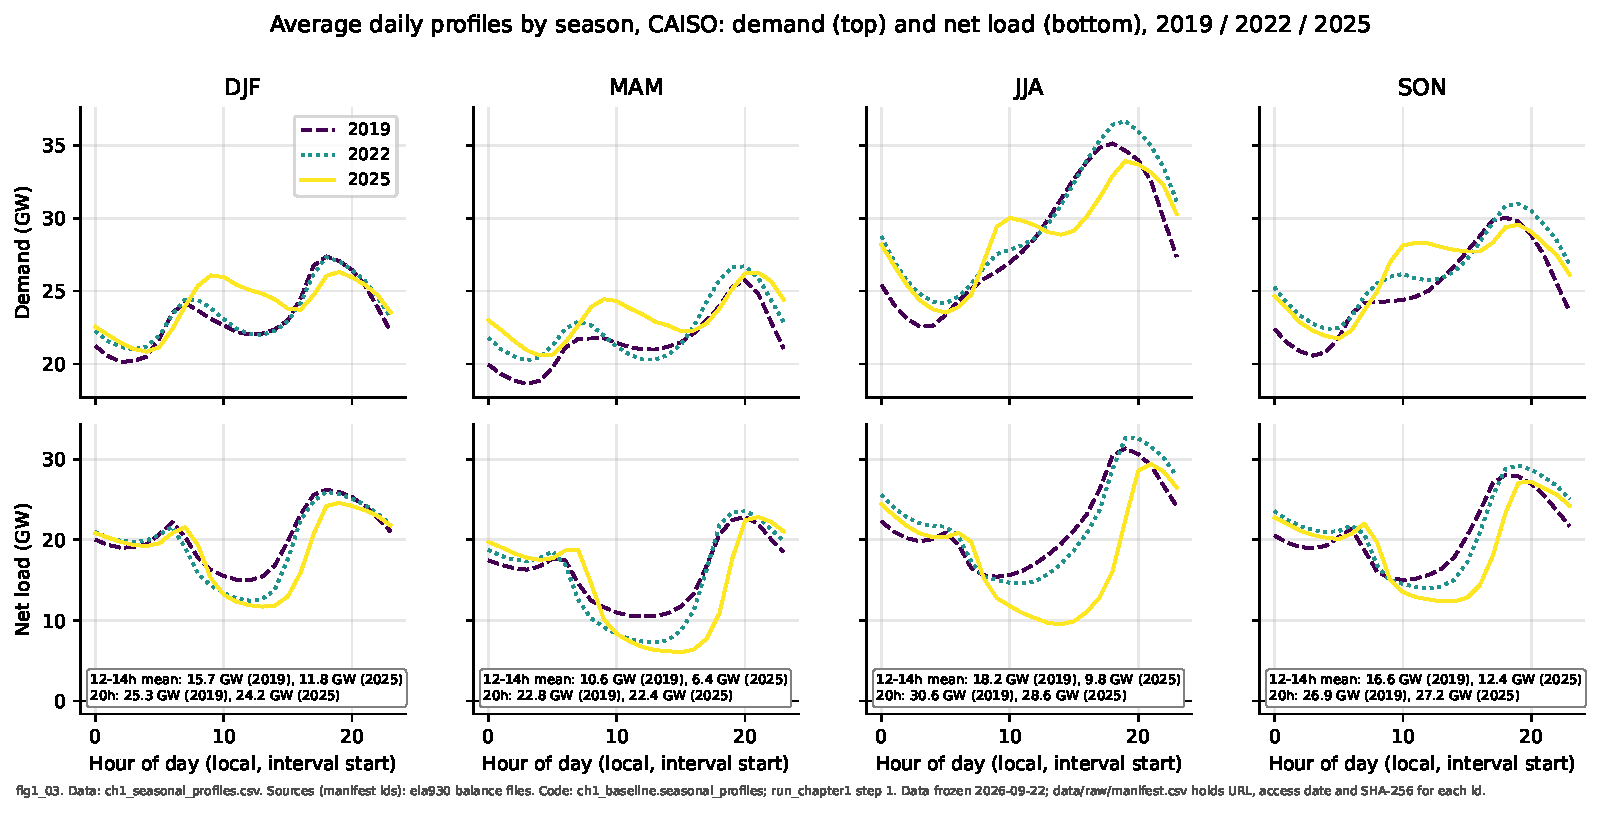
\includegraphics[width=\textwidth]{fig1_03_seasonal_daily_profiles}
\caption{Report Figure 2.3: seasonal daily profiles of CAISO demand and net load, 2019 and 2025 (source: \href{https://www.eia.gov/electricity/gridmonitor/sixMonthFiles/EIA930_BALANCE_2025_Jul_Dec.csv}{EIA-930 balance files 2019 to 2025, CISO}).}
\label{f:profiles}
\end{figure}

\paragraph{The carbon intensity drops from where to where?}
From 257 to 186~g CO$_2$ per kWh: annual energy-weighted averages of 2019 and 2025, with the peak at 277 in 2020 (Figure~\ref{f:carbon}).\src{https://www.caiso.com/outlook/history/20250701/co2.csv}{CAISO Today's Outlook daily CO$_2$ and demand history files (one CSV per day; the link opens one day)} Your intuition about the day is right and the effect is larger than the annual drop: in 2025 the spring midday intensity was 7 to 12~g/kWh against 150 to 175 in the evening, summer midday 40 to 53 against 150 to 180, winter 137 against 240 to 256. Midday is solar with gas off; the evening is gas and imports. That spread is why a flexible data center load matters: shifting the highest-intensity quarter of its hours into the lowest-intensity quarter cuts its emissions by a third (Figure~\ref{f:emissions}).

\begin{figure}[H]
\centering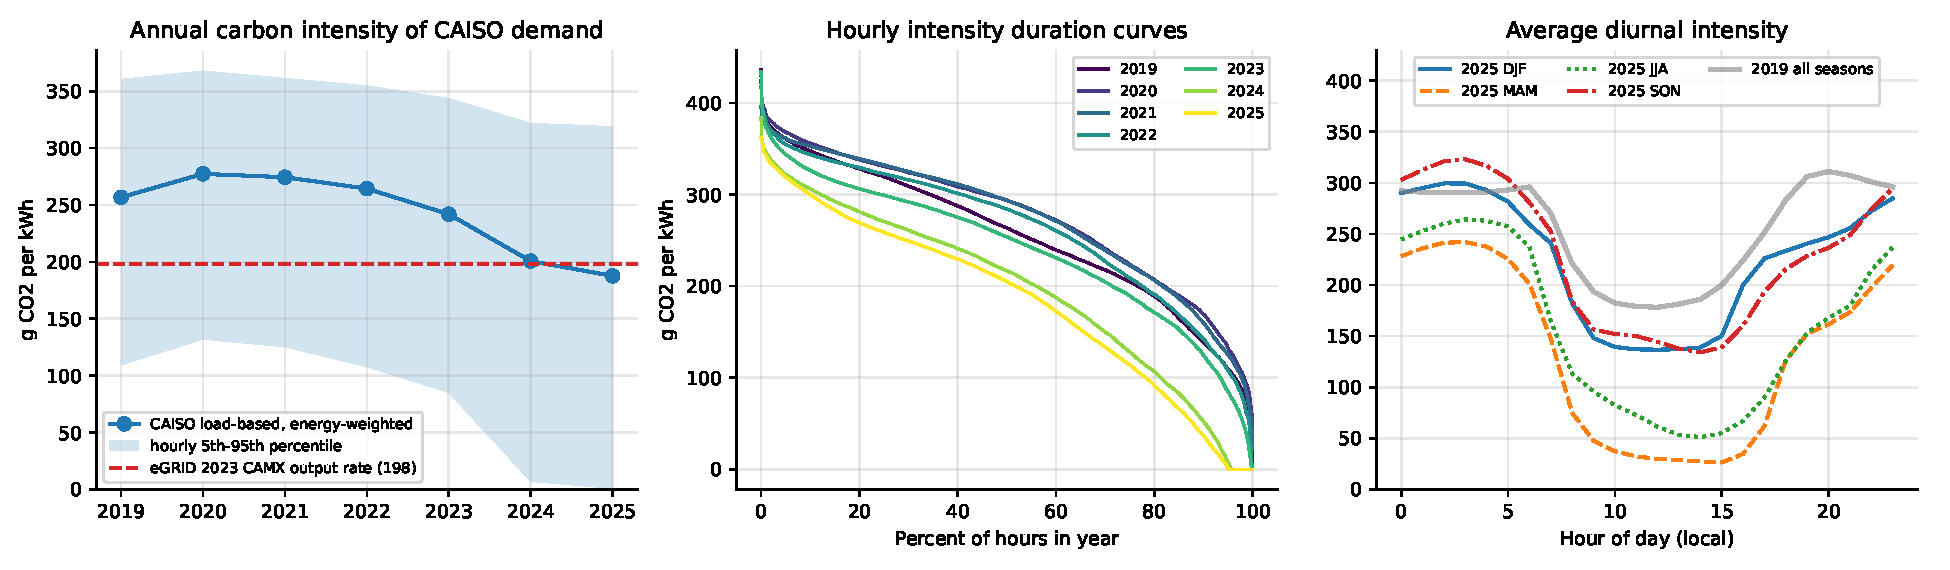
\includegraphics[width=\textwidth]{fig1_07_carbon_intensity}
\caption{Report Figure 2.7: CAISO CO$_2$ accounting intensity, annual, duration and diurnal views.}
\label{f:carbon}
\end{figure}

\paragraph{Data centers at 3 to 4 percent of California's power, and the Oregon 25 percent.}
The two are consistent. The Oregon figure comes from the ECOnorthwest and University of Virginia report of September 2026, as reported by Oregon Public Broadcasting: 111 operating data centers used about 23 percent of Oregon's retail electricity sales in 2025, with nearly 25~TWh expected by 2030.\src{https://www.opb.org/article/2026/09/17/oregon-data-centers-consume-quarter-state-power-report/}{OPB, ``Oregon data centers by the numbers'', September 17 2026, on the ECOnorthwest and University of Virginia report} Oregon's retail sales were 60~TWh in 2024 against California's 246~TWh, so 23 percent of Oregon is about 14~TWh, the same order as California's 7 to 9~TWh, which are 3 to 4 percent of a market four times larger.\src{https://www.eia.gov/electricity/data/eia861/zip/f8612024.zip}{EIA-861 2024, Sales to Ultimate Customers (parts A, C and D), computed for both states with the report's method} The Oregon-like number exists in California at the city scale: Silicon Valley Power, Santa Clara's municipal utility, reports data centers at 53 to 60 percent of its 4.5~TWh of sales.\src{https://autl.assembly.ca.gov/media/1404}{Silicon Valley Power, presentation to the Assembly oversight hearing, January 28 2026; fact sheets 2017 to 2023} The report presents the state figure as a range of four estimates because there is no metered total (Figure~\ref{f:dc}).

\begin{figure}[H]
\centering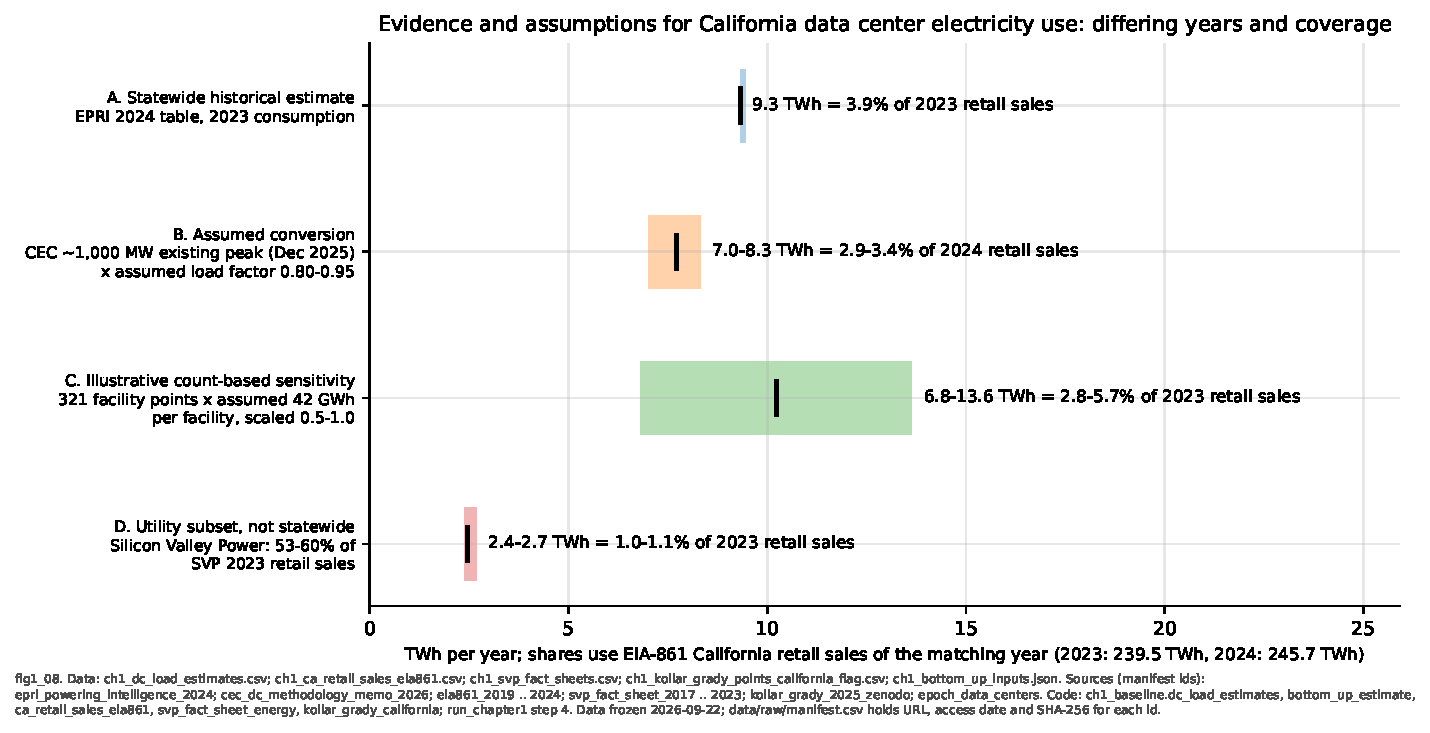
\includegraphics[width=\textwidth]{fig1_08_existing_dc_load_estimates}
\caption{Report Figure 2.8: existing data center electricity use in California, four estimates (sources: \href{https://restservice.epri.com/publicdownload/000000003002028905/0/Product}{EPRI, Powering Intelligence 2024, state table}; \href{https://www.energy.ca.gov/sites/default/files/2026-04/Data_Center_Methodology_Memo_ada.pdf}{CEC methodology memo}; \href{https://autl.assembly.ca.gov/media/1404}{SVP}).}
\label{f:dc}
\end{figure}

\paragraph{No uptick in California after 2022?}
Not in the physical indicators, and that is the finding rather than a puzzle. The national Census series is construction spending on data centers (Figure~\ref{f:census}); it rose from USD 1.6 billion a year in January 2014 to 75.2 billion in July 2026, and the break located by the data is March 2022, after which the series grew 61 percent a year until mid-2024 and 36 percent since.\src{https://www.census.gov/construction/c30/xlsx/privsatime.xlsx}{Census Bureau, Value of Construction Put in Place, private, seasonally adjusted (privsatime.xlsx), data center line} California's own indicators did not follow (Figure~\ref{f:proxies}). Employment in computing infrastructure, data processing and hosting (QCEW industry 518210) grew 12 percent a year to 74,000 jobs by the end of 2022, stepped to 84,000 in the first quarter of 2023 and has been flat since (84,000 in the first quarter of 2026);\src{https://data.bls.gov/cew/data/api/2026/1/industry/518210.csv}{BLS Quarterly Census of Employment and Wages, NAICS 518210, California, quarterly files 2014 to 2026 Q1} Silicon Valley colocation capacity under construction has stayed between 125 and 168~MW since 2023;\src{https://e.infogram.com/19516a4e-2f1e-4319-ad1e-5c3afc080c41}{CBRE North America Data Center Trends, Silicon Valley market chapters (Infogram tables), H2 2025 and H1 2026} and Epoch AI's satellite-tracked hub lists 75 large United States AI sites, led by Texas, Virginia, Ohio and Iowa, with none in California.\src{https://epoch.ai/data/data_centers/data_centers.csv}{Epoch AI, Frontier Data Centers Hub, data\_centers.csv (snapshot of September 22 2026)} What rose in California is requests to connect: the CEC's like-for-like count of signed agreements plus applications at PG\&E and SCE went from 6,771~MW in December 2024 to 11,219~MW in December 2025, and the full three-tier count reached 20,677~MW in the state (Figure~\ref{f:tiers}).\src{https://www.energy.ca.gov/sites/default/files/2026-04/Data_Center_Methodology_Memo_ada.pdf}{CEC, Data Center Methodology Memo, April 2026, Table 1; preliminary forecast deck of October 30 2025, slides 6 and 7} The uptick is on paper; the physical build is going where power and land are available.

\begin{figure}[H]
\centering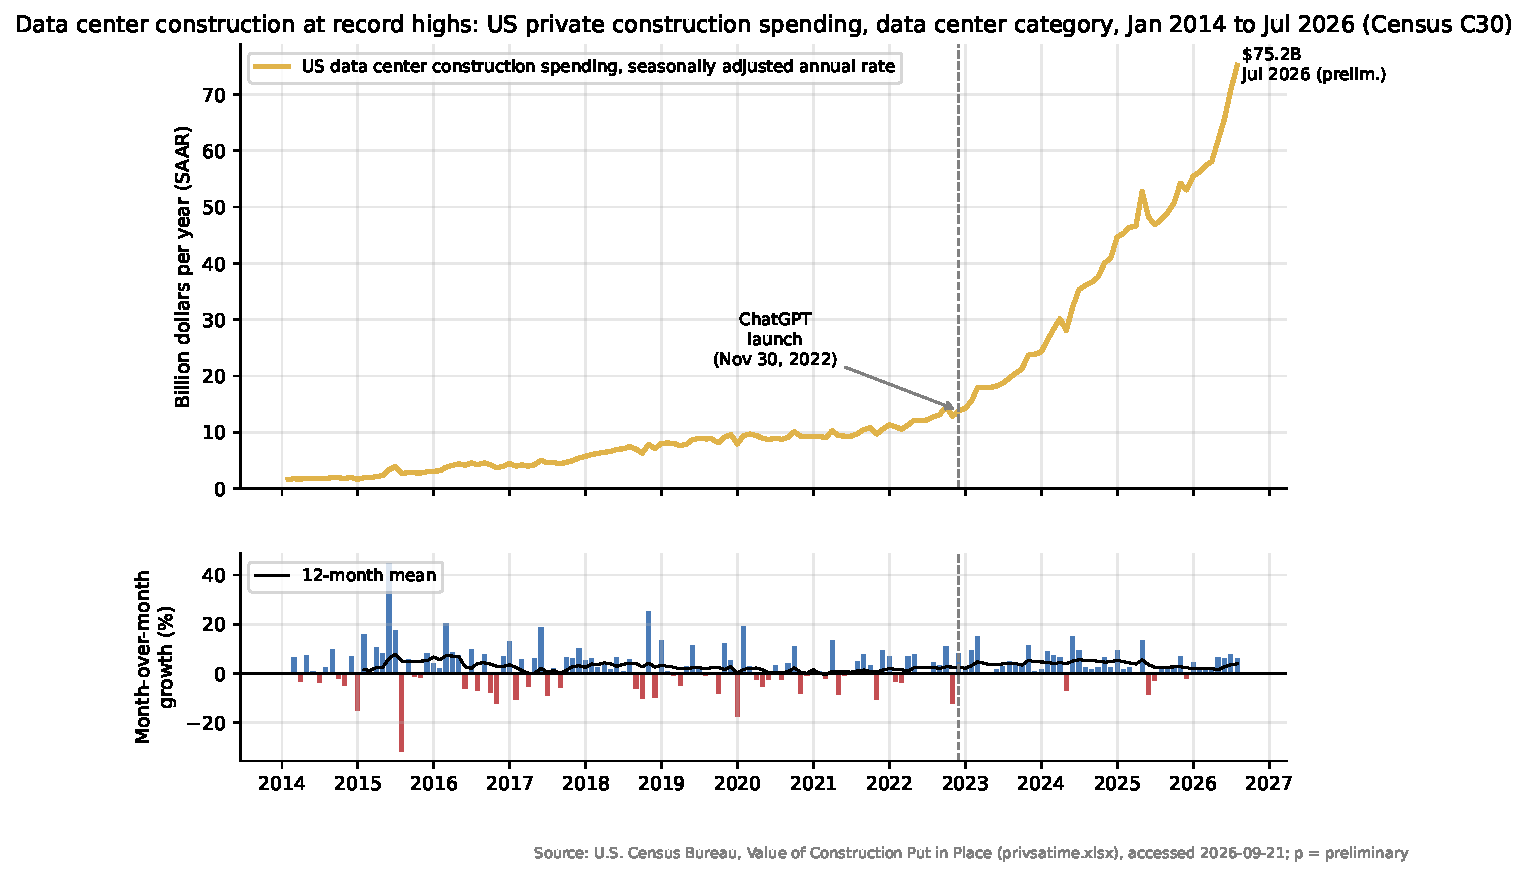
\includegraphics[width=\textwidth]{fig2_01_census_data_center_construction}
\caption{Report Figure 3.1: US private data center construction spending, with the ChatGPT release marked.}
\label{f:census}
\end{figure}

\begin{figure}[H]
\centering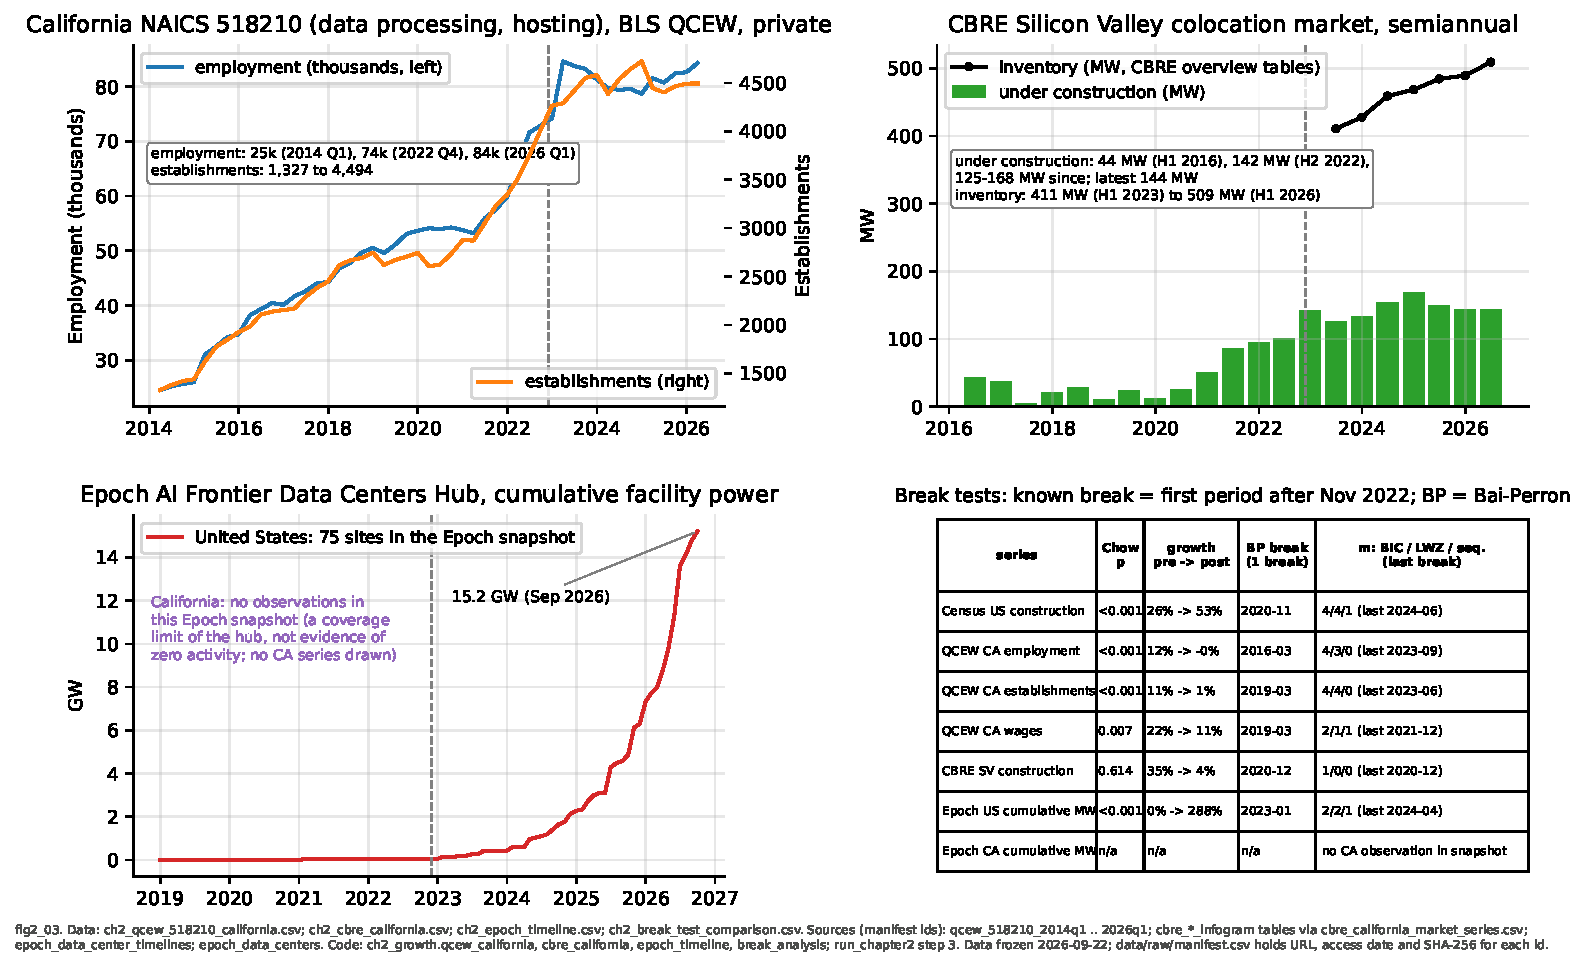
\includegraphics[width=\textwidth]{fig2_03_california_proxies}
\caption{Report Figure 3.3: California proxies, QCEW employment and establishments, CBRE Silicon Valley construction and inventory, Epoch AI sites, and the break-test summary.}
\label{f:proxies}
\end{figure}

\paragraph{The SCE numbers.}
SCE is the only utility that publishes its request list project by project, twice so far, in August 2025 and January 2026.\src{https://efiling.energy.ca.gov/GetDocument.aspx?tn=268459}{SCE, IEPR 2025 Data Center Database (public), January 29 2026, TN 268459; the August 29 2025 edition is TN 266008} Between the two snapshots the active requests fell from 6,201 to 5,162~MW while the cumulative cancelled amount rose from 709 to 3,137~MW: 2.4~GW of requests were cancelled in five months even as new ones arrived. The same list shows advancement, since the inquiry tier fell from 5,934 to 1,773~MW while the application tier grew from 216 to 3,313~MW. So the pipeline churns in both directions, and about 38 percent of everything SCE has ever recorded is now cancelled. That churn is the empirical reason to discount requests rather than count them (Figure~\ref{f:tiers}; report Table 3.9).

\begin{figure}[H]
\centering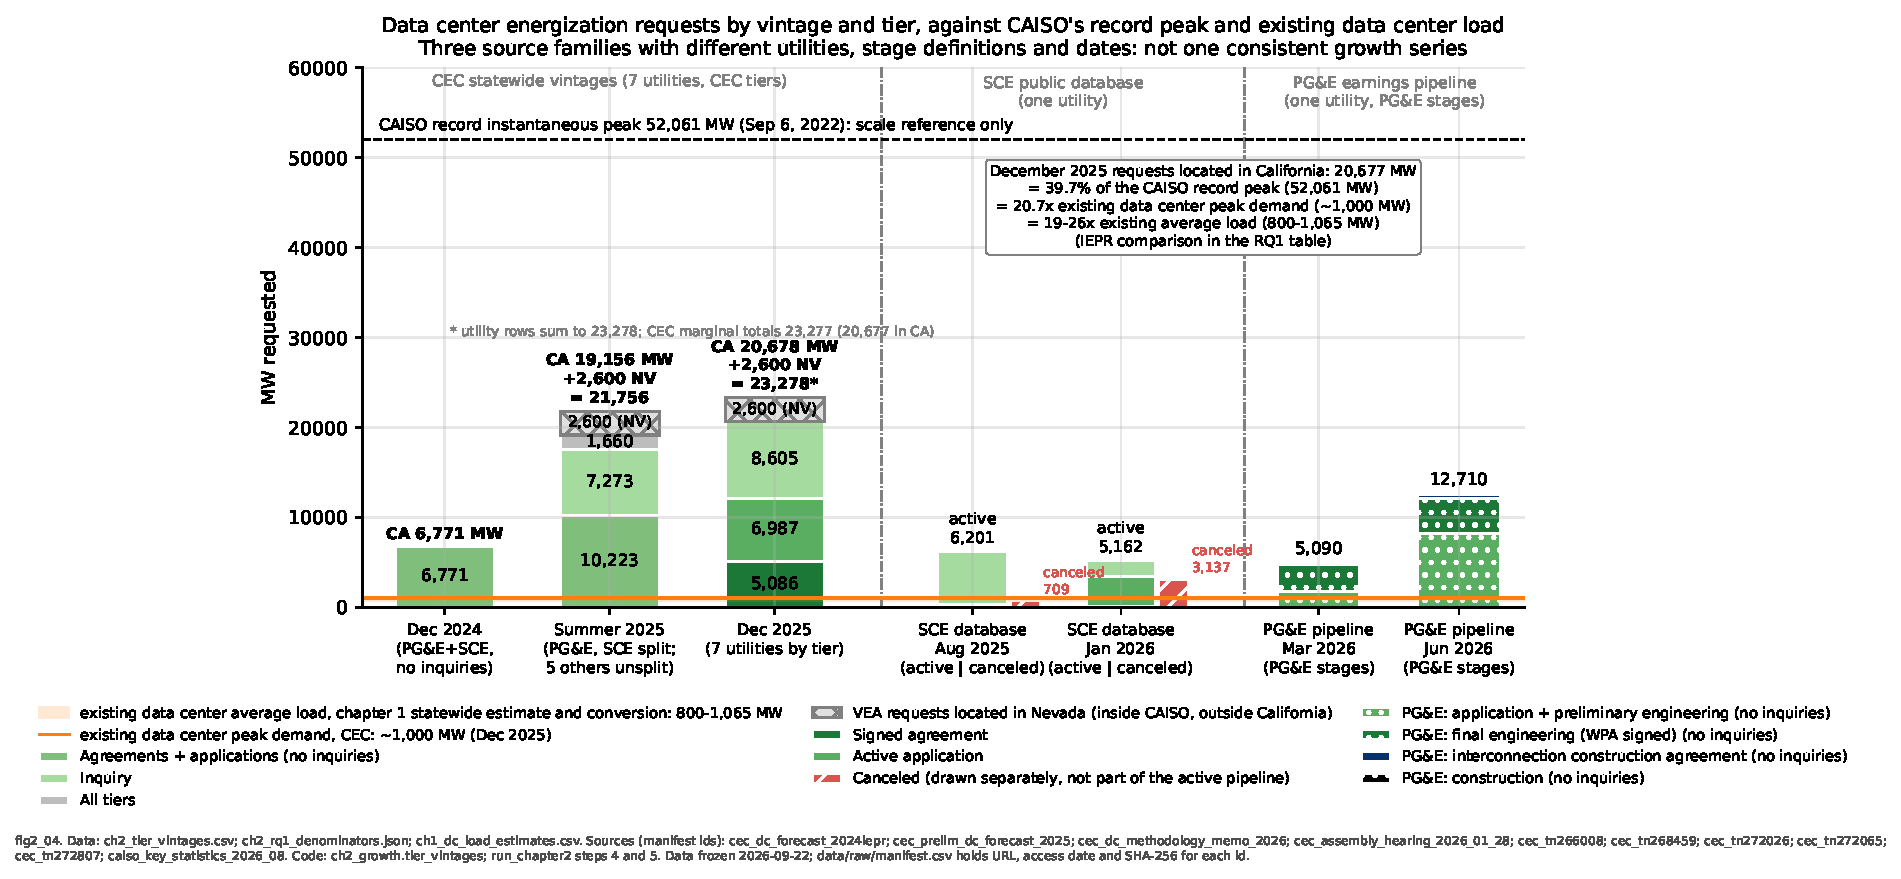
\includegraphics[width=\textwidth]{fig2_04_tier_vintages}
\caption{Report Figure 3.4: energization requests by vintage and tier against the grid, with Nevada separated and SCE's cancellations shown (sources: \href{https://autl.assembly.ca.gov/media/1402}{CEC presentation to the Assembly oversight hearing, January 28 2026}; \href{https://www.caiso.com/documents/key-statistics-aug-2026.pdf}{CAISO Key Statistics, August 2026}).}
\label{f:tiers}
\end{figure}

\paragraph{Forty percent of peak; what share of the total?}
Because a data center runs flat, the energy comparison is the stronger one and the report carries both (Table 3.10). If all 20,677~MW ran flat at full capacity they would draw 181~TWh a year, 81 to 84 percent of CAISO's 216 to 224~TWh of annual demand and 69 percent of the state's 263~TWh;\src{https://efiling.energy.ca.gov/GetDocument.aspx?tn=268727}{CEC, CED 2025 Planning forecast, Form 1.5a (statewide energy to serve load 2025 and 2030)} at the CEC's 67 percent utilization and an 88 percent load factor, 107~TWh, three times the state's forecast energy growth to 2030. The signed tier alone, 5,086~MW, would draw 45~TWh flat, a fifth of CAISO's demand. The CEC's own probability-weighted central case is 12~TWh in 2030, 4 percent of the 298~TWh the state forecasts for that year.\src{https://efiling.energy.ca.gov/GetDocument.aspx?tn=268824}{CEC, CED 2025 Planning forecast, Form 1.1c data center allocations, TN 268824}

\paragraph{California-only headline, or other states?}
The headline stays California-only (20,677~MW, with the 2,600~MW that Valley Electric reported for Nevada as a memo line and the CEC's 23,277~MW total beside it). No consistent 50-state series exists, which is itself a finding of the regime comparison. Two other regions enter as data (Figure~\ref{f:ercot}): ERCOT publishes its queue monthly by phase, 63~GW of requests in December 2024 and 467~GW by July 2026 against 9.5~GW approved to energize and about 4~GW observed operating,\src{https://www.ercot.com/files/docs/2026/08/17/ERCOT-Monthly-Operational-Overview-July-2026.pdf}{ERCOT, Monthly Operational Overview, July 2026, slides 9 and 10; ERCOT Monthly, July 2025 (63 GW in December 2024)} and PJM publishes an explicit firm and non-firm rule with 33.7~GW of large-load adjustments in its 2030 forecast.\src{https://www.pjm.com/-/media/DotCom/planning/res-adeq/load-forecast/2026-load-report-tables.xlsx}{PJM, 2026 Load Forecast Report tables, Table B-9; Load Adjustment Requests Summary, November 24 2025} Oregon can be added as a comparison row from the ECOnorthwest report if you would like it.

\begin{figure}[H]
\centering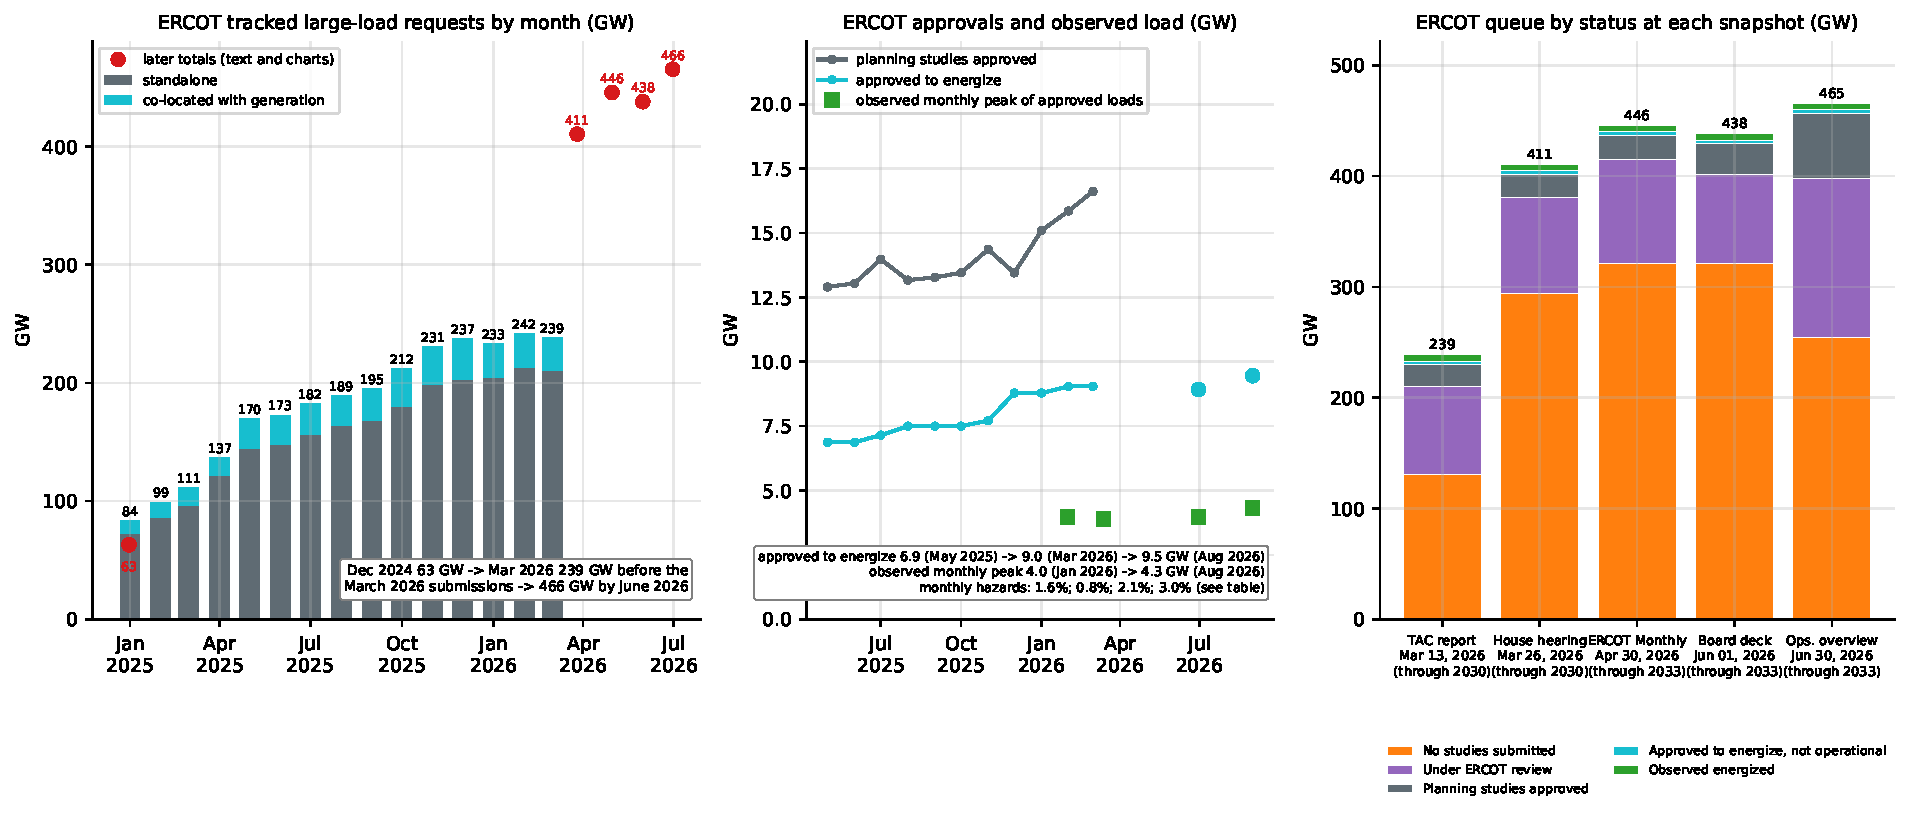
\includegraphics[width=\textwidth]{fig4_05_ercot_queue}
\caption{Report Figure 5.6: ERCOT's large-load queue by month, approvals and observed load, and the queue by status at each 2026 snapshot.}
\label{f:ercot}
\end{figure}

\paragraph{``How far should the confidence factors carry above the cancellation signals?''}
What I meant: the CEC assigns fixed probabilities that a request in each tier is built (70, 33 and 0 percent in its central case), while SCE's cancellations and ERCOT's slow phase transitions suggest lower values.\src{https://www.energy.ca.gov/sites/default/files/2026-04/Data_Center_Methodology_Memo_ada.pdf}{CEC, Data Center Methodology Memo, April 2026, Table 2 (confidence levels, utilization, ramp)} The statistical content is in Chapter 5 of the report: the CEC's probabilities are treated as uncertain inputs bracketed by the CEC's own two cases, by rates estimated from ERCOT's monthly queue (37, 6 and 2 percent over five years) and by PJM's firm-only rule, and 10,000 Monte Carlo draws propagate them together with the supply side (Figure~\ref{f:gap}). The answer is that the question matters less than it seemed: the three tier probabilities together explain about 2 percent of the variance of the 2030 energy gap and 4 percent of the peak gap. Imports, the state's own load forecast, hydro and Diablo Canyon explain most of it (Figure~\ref{f:sens}).

\begin{figure}[H]
\centering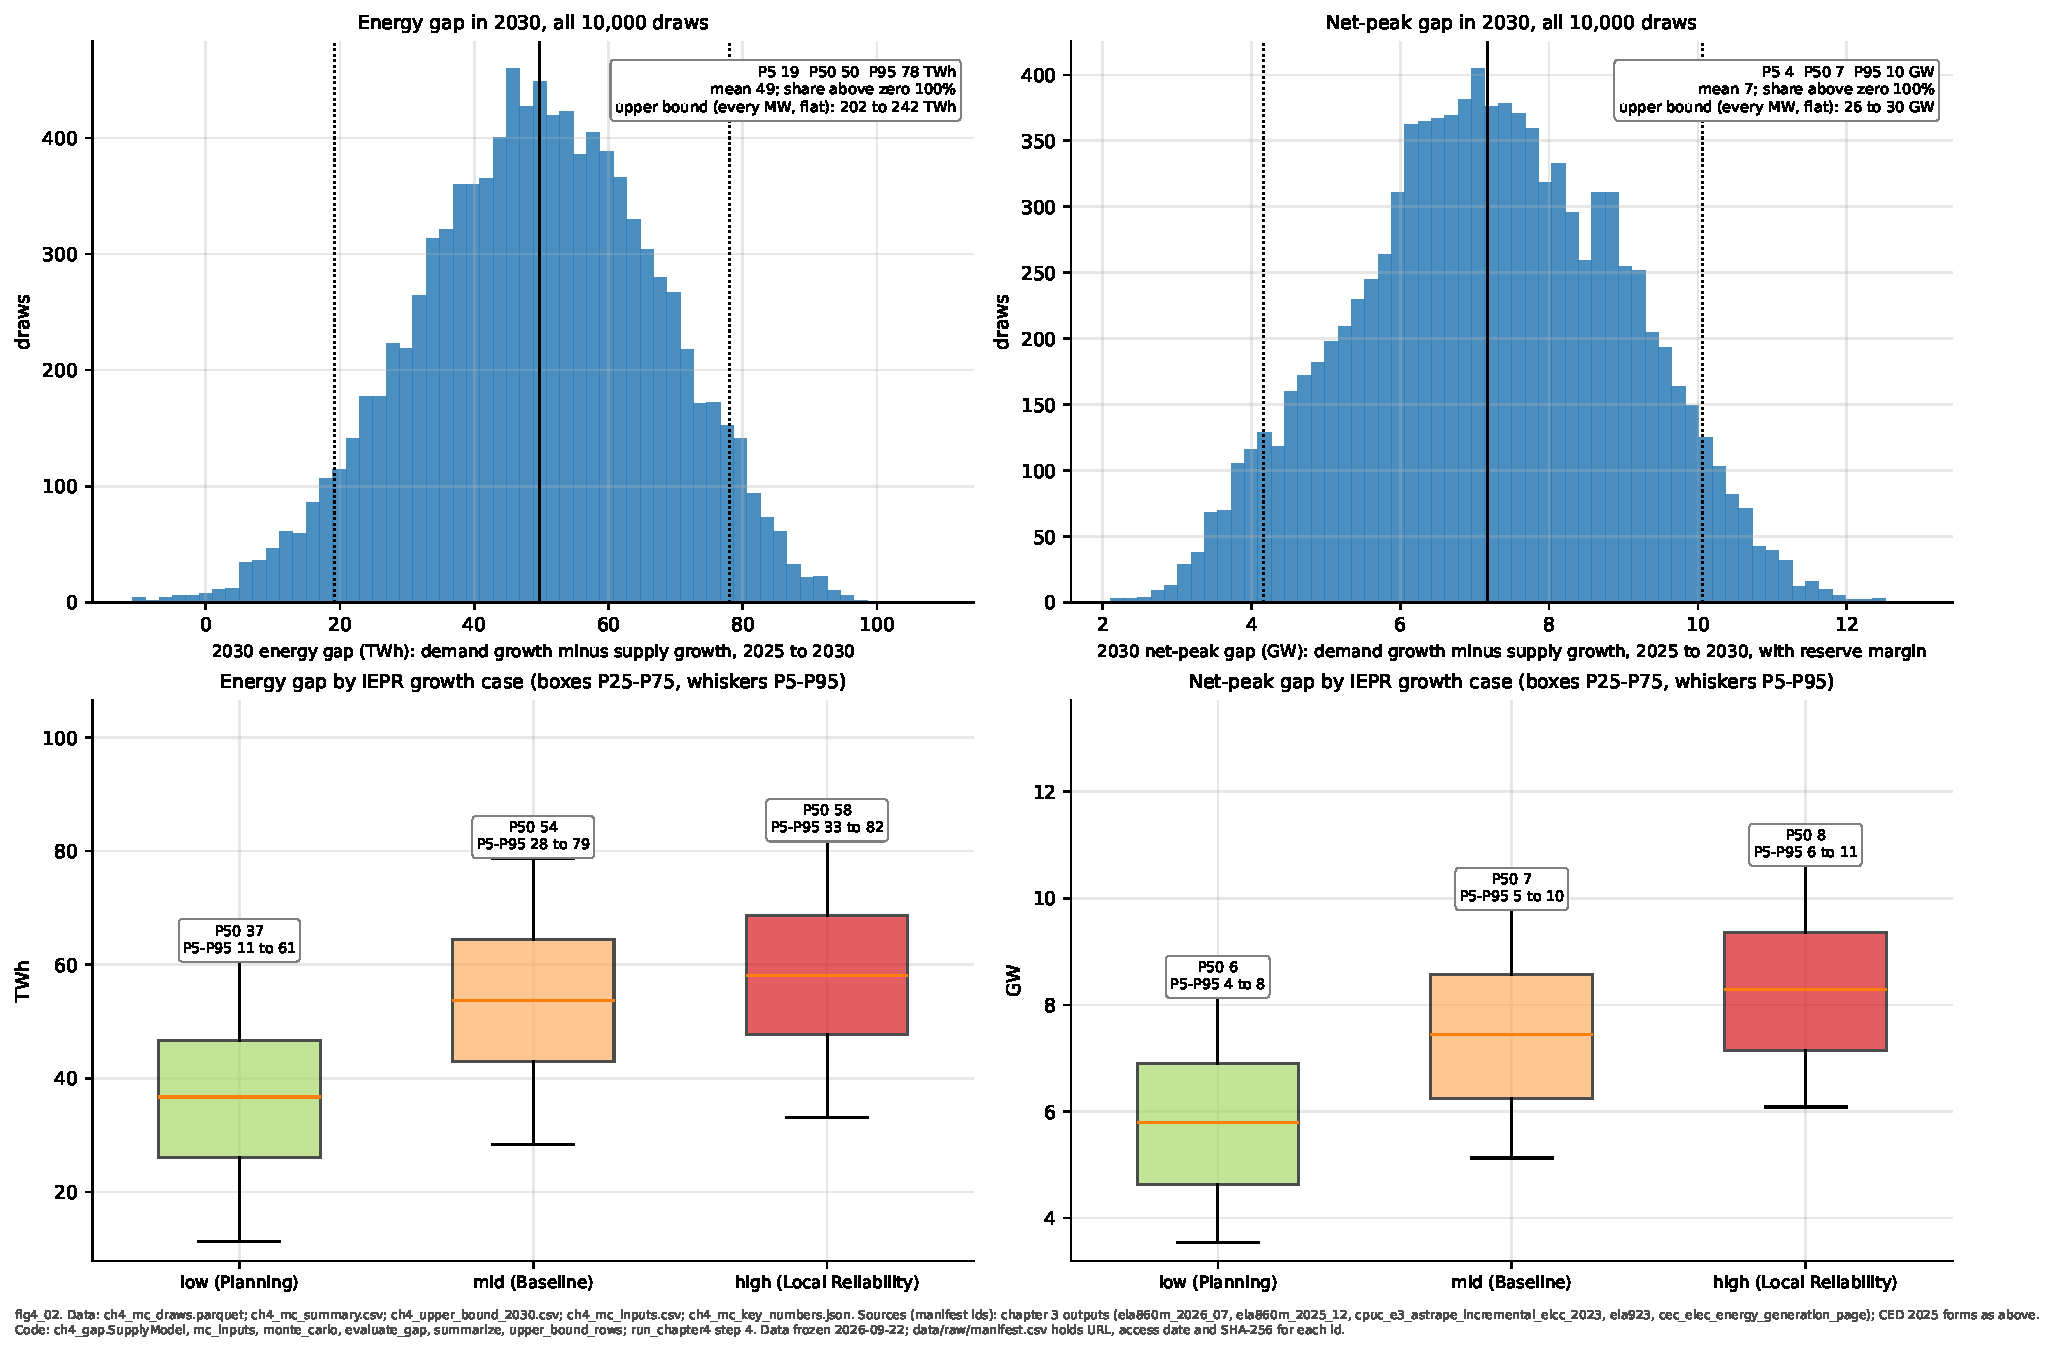
\includegraphics[width=\textwidth]{fig4_02_gap_distributions}
\caption{Report Figure 5.2: the 2030 energy and net-peak gap over 10,000 draws.}
\label{f:gap}
\end{figure}

\begin{figure}[H]
\centering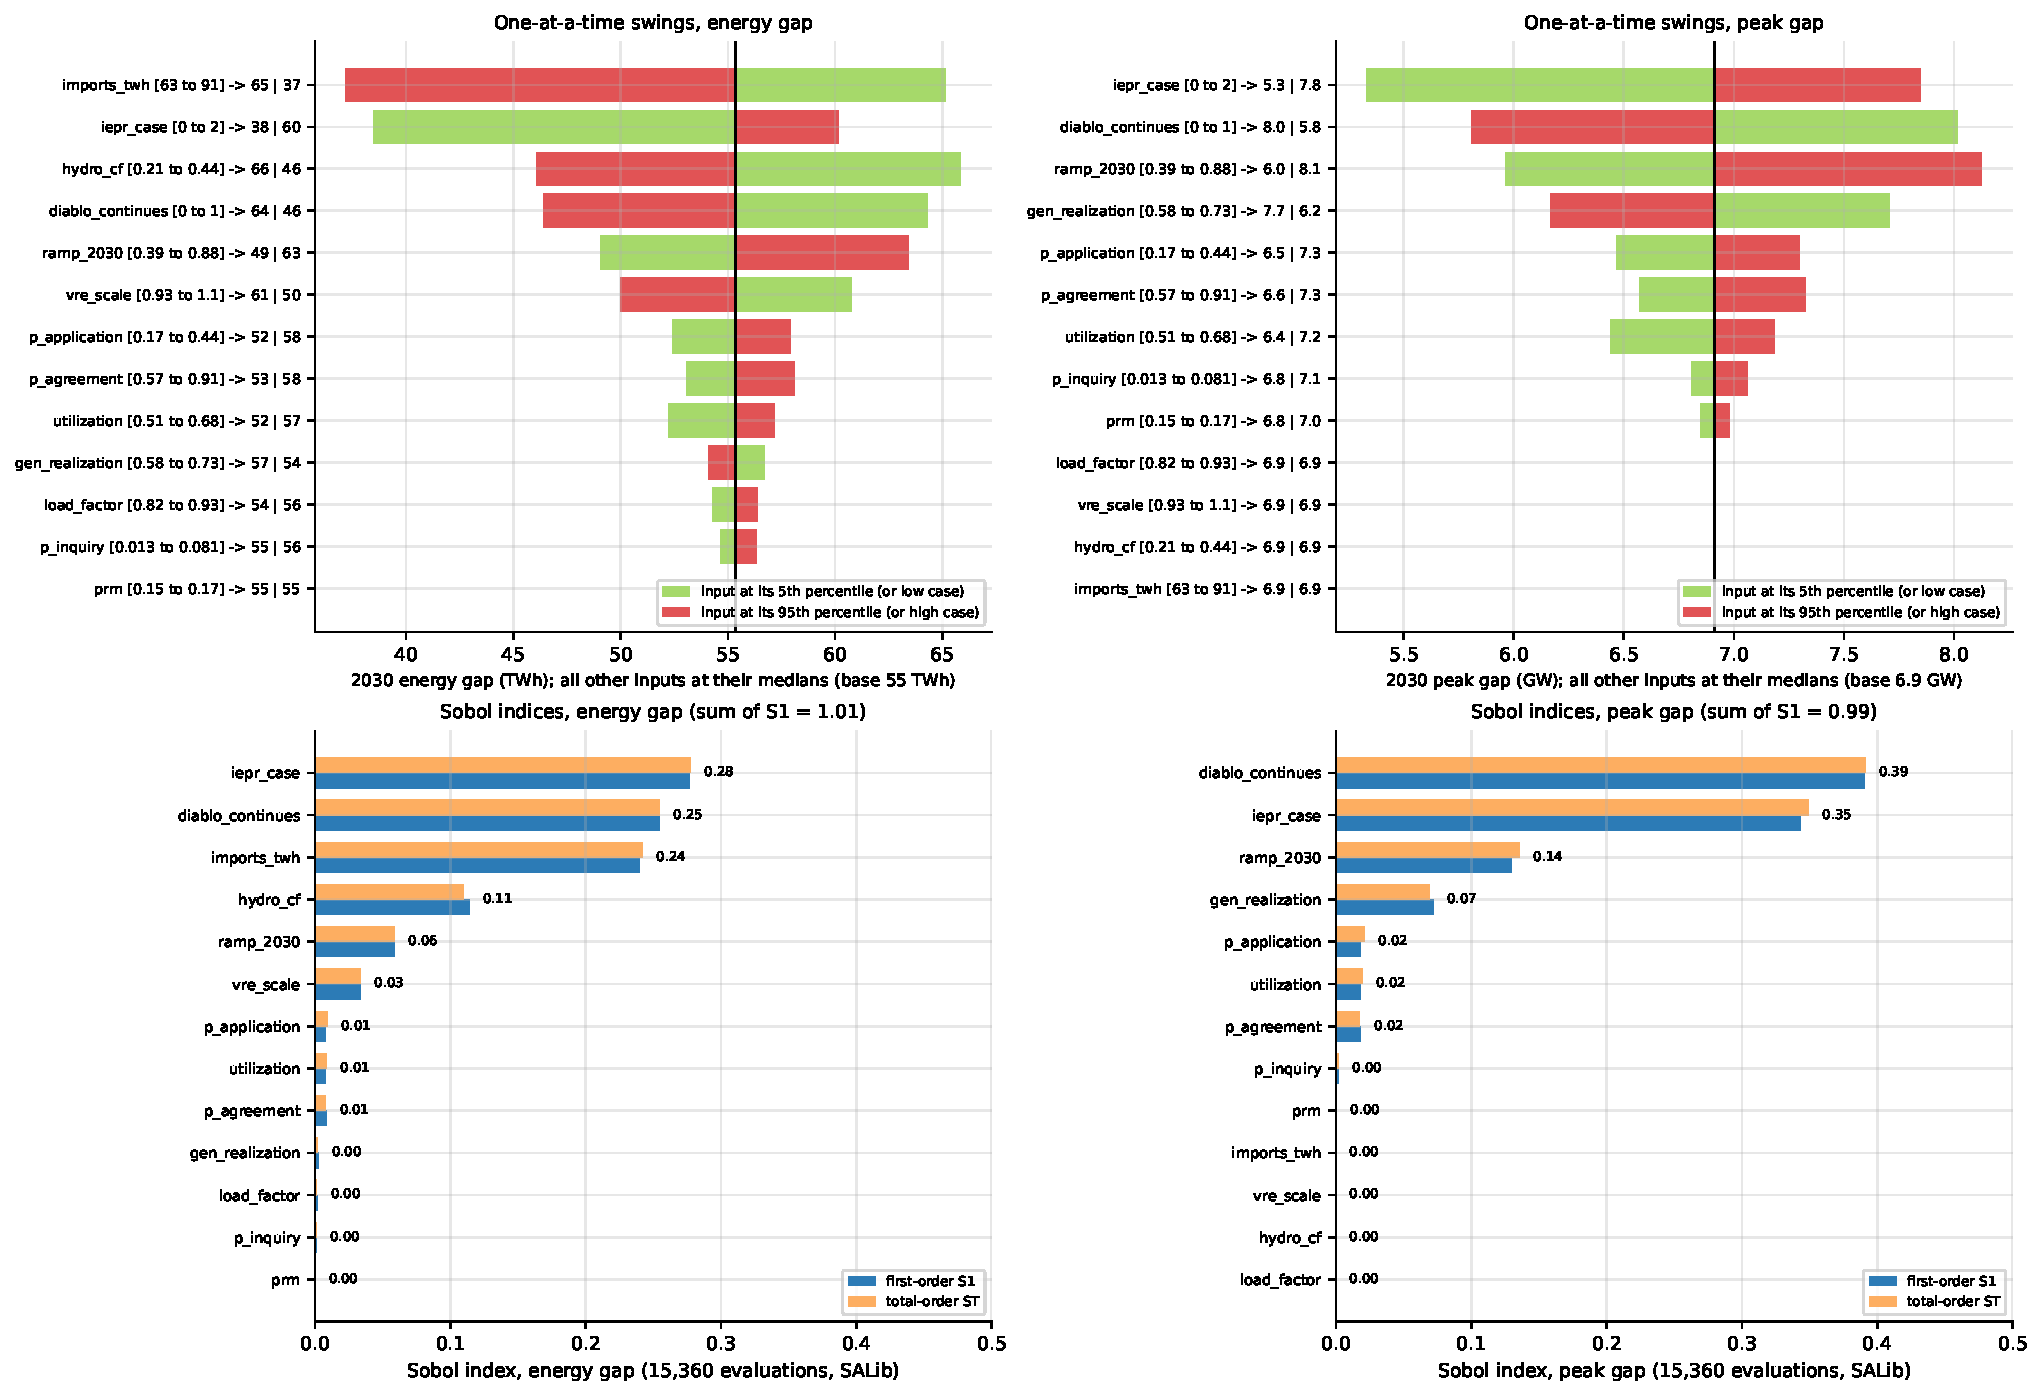
\includegraphics[width=\textwidth]{fig4_03_sensitivity}
\caption{Report Figure 5.3: one-at-a-time swings and Sobol indices for both gaps.}
\label{f:sens}
\end{figure}

\begin{figure}[H]
\centering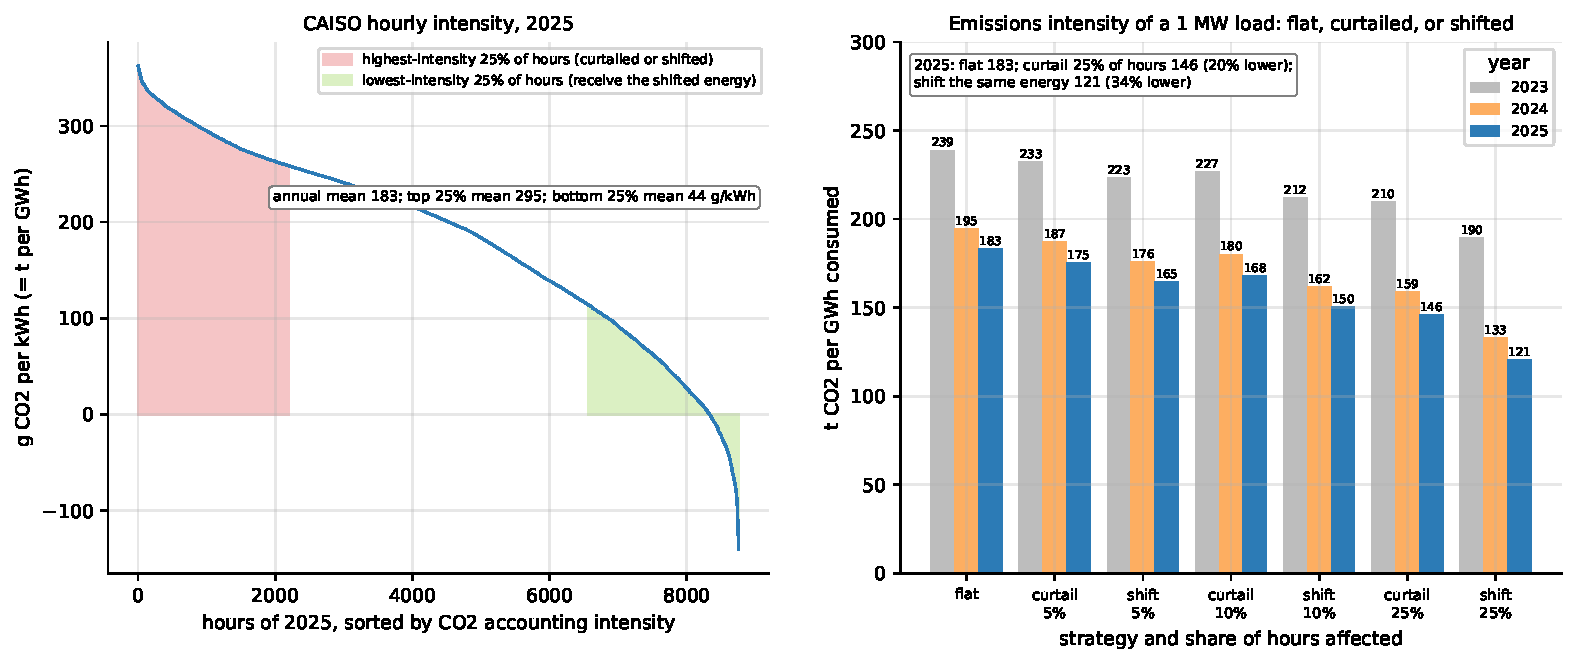
\includegraphics[width=\textwidth]{fig4_06_emissions_flat_vs_flexible}
\caption{Report Figure 5.7: emissions of a flat, curtailed or shifted 1~MW load on CAISO's hourly intensity.}
\label{f:emissions}
\end{figure}

\section*{Corrections to my September 22 email}
\begin{itemize}
\item The CAISO record peak of 52,061~MW was set on September 6, 2022, not in October 2023.\src{https://www.caiso.com/documents/key-statistics-aug-2026.pdf}{CAISO, Key Statistics, August 2026}
\item ``Midday averaged out at 6~GW and evening unchanged at 22~GW'' is the spring profile (12:00 to 14:00 net load 6.4~GW in 2025 from 10.6 in 2019; 20:00 net load 22.4~GW). Across all seasons the midday mean fell from 15.3 to 10.1~GW and the evening from 26.4 to 25.6~GW (Figure~\ref{f:profiles}).
\item ``Requests increased from 6,771 to 23,277~MW'' compares two different counts. Like for like (agreements plus applications, PG\&E and SCE) the increase is 6,771 to 11,219~MW; the 23,277~MW is all three tiers at seven utilities and includes Nevada.
\item Midday prices in 2025 averaged USD 13 per MWh at the SCE point and 24 to 26 at the PG\&E point (11:00 to 14:00); evening prices (18:00 to 20:00) averaged 49 to 56. The ranges I quoted mixed years and nodes.\src{https://oasis.caiso.com/oasisapi/SingleZip?queryname=PRC_LMP&market_run_id=DAM&version=12}{CAISO OASIS, day-ahead locational marginal prices, PRC\_LMP DAM, default load aggregation points}
\end{itemize}

\section*{How the work is organized for you}
The Overleaf project holds the report (\texttt{main.tex}), this memo (\texttt{brief.tex}) and the 21-slide deck (\texttt{defense.tex}); switch the main document in the Overleaf menu to compile each. The report opens with a one-page summary for the reader and a glossary, then one chapter per phase, then the discussion and two provenance appendices; Appendix B lists the URL, access date and checksum behind every source a figure names. I will keep the project current and add a dated ``what changed'' note at the top before each meeting. The repository, raw data and processed files stay on my side.

\section*{Meetings}
Wednesdays at noon on campus suits me, progress-dependent as you suggest, with Zoom on Tuesdays or Thursdays when something cannot wait. I will send a short update the day before each meeting.

\section*{Next steps}
Revise the discussion with your comments; add Oregon and the CEC's 2026 IEPR vintage when it appears; keep the monthly snapshots of the ERCOT queue and the CEC docket running so that California's own transition rates can be estimated next year; prepare the defense.
\end{document}
